% !TeX root = ../thesis.tex
\chapter{Existence of Kink-Like Traveling Wave Solutions}
\label{chp:existence}
\pagestyle{myheadings}

\section{Introduction}

The goal of this chapter is to show the existence of the traveling wave solution for the FPUT lattice and describe its profile. From formal calculations and the numerical experiments carried out in \cite{pace2019beta}, it seems that the traveling wave solution has a profile given by the kink solution to the defocusing mKdV, \cref{intro-defocusing-mkdv}; that is, for \(\varphi_1(\cdot) = \frac 1 {\sqrt 2} \tanh(\cdot/\sqrt 2)\) we expect to have a traveling wave solution \(u\) such that 
\begin{equation}\label{formal-approximation}
	u_n(t) = \epsilon \varphi_1(\epsilon(n - ct)) +\mcO(\epsilon^3)
\end{equation}
when \(c\) is slightly smaller than \(V''(0) = 1\).

One would expect that methods used to find the solitary wave solution for the FPUT can also be applied to this case. Notably it was shown in \cite{friesecke1999solitary} that there exists a solitary wave solution whose profile is described by the KdV soliton using a fixed-point argument. The argument relies on creating a map from \(H^1(\R)\) to itself using Fourier multipliers such that the fixed point of the map is the profile of the solitary wave. However, this argument does not seem to extend to our case since the function \(\varphi_1\) is not in a Sobolev space and its Fourier transform is defined only in a distributional sense. Due to this problem, we neglect the functional approach and focus on techniques from bifurcation theory. 

One common technique for constructing traveling wave solutions to PDEs is by using the center manifold theorem. For PDEs of one spatial and one temporal variable, the strategy is to assume that the solution is a traveling wave (i.e.\ of the form \(f(x-ct)\)) to eliminate the derivative with respect to \(t\) and reduce the problem to an ODE with respect to the spatial variable \(x\). Finding bounded solutions of this ODE then results in traveling wave solutions of the PDE. The center manifold is an important tool for finding these solutions since (1) it is typically finite-dimensional, (2) can be approximated by Taylor series up to arbitrary order, and (3) contains all bounded solutions. If a linear operator has an eigenvalue pass through the line \(\{\lambda\in\mathbb C: \Re \lambda = 0\}\) as a parameter \(\mu\) varies, then one can have a center manifold containing small bounded solutions parameterized by \(\mu\). Similar techniques can be used to find center manifold for more general semi-dynamical systems defined on Banach spaces \cite{vanderbauwhede1992center}. Such a construction was carried out in \cite{iooss2000travelling} for an abstract ODE representing an advance delay differential equation. The existence of several traveling wave solutions on the FPUT lattice were proved. The bifurcation parameter in this paper was given in part by the wave speed. In fact, \cite[Thm.\ 5]{iooss2000travelling} shows the existence of a heteroclinic orbit on the center manifold when \(c\) is slightly smaller than \(1\). This heteroclinic orbit corresponds to the kink-like solution of the FPUT we are interested in. But no description of its wave profile was given, so obtaining an estimate of the form in \cref{formal-approximation} is still an open problem.


Our argument for getting such an estimate will proceed as follows. We first follow the procedure in \cite{iooss2000travelling}
to construct the center manifold parameterized by \(\epsilon\), making sure to explicitly compute the dynamics on the center manifold. Making a suitable change of variables, we look for small-amplitude, long-wavelength solutions for the FPUT on the center manifold and show that formally setting \(\epsilon = 0\) gives a solution related to the kink solution \(\varphi_1\). Next we apply results from Fenichel theory to show that this solution persists for \(\epsilon> 0\). Lastly we convert our results back to the original formulation of the FPUT lattice and prove an estimate of the form \cref{formal-approximation}.


%Main result here?

\section{Construction of Center Manifold}
%Change of coordinates to get into the form of an abstract ODE.
We follow the construction of the center manifold carried out in \cite{iooss2000travelling}. Recall that the equations for the FPUT lattice are given by
\begin{equation*}
	\ddot x_n = V'(x_{n+1} - x_n) - V'(x_n - x_{n-1}), \quad n \in \Z. \tag{\ref{fput-lattice-odes}}
\end{equation*}
We assume that \(V(x) = \frac 12 x^2 - \frac 1 {24} x^4 + \mcO(x^5)\) near \(x=0\). This choice of potential is chosen so that \(V''(0) = 1\) and \(V^{(4)}(0) = -1\); if we have a potential where \(V(0) = V'''(0)=0\), \(V''(0) > 0\) and \(V^{(4)}(0)< 0\), we can rescale to get the potential above. We make the ansatz that 
\begin{equation*}
	x_n(\tilde t) = x(n-c\tilde t),
\end{equation*}
where the \(x(t)\) on the right is a function from \(\R\) to \(\R\). Hence \(x(t)\) must satisfy the advance-delay differential equation
\begin{equation}\label{advance-delay-equation}
	\ddot x (t) = \mu \Big(V'(x(t+1) - x(t)) - V(x(t) - x(t-1)) \Big)
\end{equation}
where \(\mu = c^{-2}\). For delay differential equations like the one above, we are inherently working with an infinite-dimensional problem; the dynamics of \(x(t)\) are determined by its value on an interval of \(t\). Instead of working directly with \cref{advance-delay-equation}, we rewrite the equation as a first-order differential equation in a Banach space. \Cref{advance-delay-equation} cannot be written as a differential equation in a finite-dimensional phase space, and so we use a Banach space to represent a ``slice'' of the function on the interval \([t-1,t+1]\) for \(t\in\R\). We introduce a new variable \(v\in[-1,1]\) and functions \(X(t,v) = x(t+v)\). We use the notation \(\xi(t) = \dot x(t)\), \(\delta^1X(t,v) = X(t,1)\), and \(\delta^{-1} X(t,v) = X(t,-1)\). Then letting \(U(t) = (x(t), \xi(t), X(t,v))^T\) represent our solution, \cref{advance-delay-equation} can be written as follows:
\begin{equation}\label{first-order-abstract-ode}
	\partial_t U = L_\mu U + M_\mu (U)
\end{equation}
where \(L_\mu\) is the linear operator %Explain \partial_\nu. Corresponds to shift, but how do we get unique solutions?
\begin{equation*}
	L_\mu = \begin{pmatrix}
		0 & 1 & 0\\
		-2\mu & 0 & \mu(\delta^1 + \delta^{-1}) \\
		0 & 0 & \partial_v
	\end{pmatrix}
\end{equation*}
and 
\begin{equation*}
	M_\mu(U) = \mu (0, g(\delta^1X -x) - g(x- \delta^{-1} X), 0)^T
\end{equation*}
where we define \(g(x)= V'(x) - x\). Note the second component of \cref{first-order-abstract-ode} corresponds with the advance-delay equation. The third component corresponds to the functional part  \(X(t,\nu)\) and gives \(\partial_t X = \partial_\nu X\), so that the solution is given by a translation . We will also require that \(X(t,0) = x(t)\), so that \(X(t,v) = x(t+v)\) and solutions of \cref{first-order-abstract-ode} correspond with solutions of \cref{advance-delay-equation}. We introduce the following Banach spaces for \(U\):
\begin{equation*}
	\begin{aligned}
		\bbH &= \R^2 \times C[-1,1] \\
		\bbD &= \{(x, \xi, X) \in \R^2 \times C^1[-1,1] \mid X(0) = x\}
	\end{aligned}
\end{equation*}
where the spaces have the usual maximum norms. The operator \(L_\mu\) is continuous from \(\bbD\) to \(\bbH\). Assuming that \(g\in C^4(I)\) where \(I\) is an open neighborhood around \(0\), we have \(M_\mu \in C^4(\bbD,\bbD)\).

The system above has a reversibility symmetry \(S\) given by 
\begin{equation*}
	S(x, \xi, X)^T = (-x, \xi, -X \circ s)^T
\end{equation*}
where \(X\circ s (v) = X(-v)\). That is, \cref{first-order-abstract-ode} is reversible and if \(U(t)\) is a solution then so is \((S\circ U)(-t)\). Additionally, if \(V'(x)\) is odd, then \cref{first-order-abstract-ode} is also odd; this means that if \(U(t)\) is a solution then so is \(-U(t)\).

Note that \cref{first-order-abstract-ode} does not have all solutions in \(\mathbb D\) and so some may not correspond with the requirement that \(X(t,0) = x(t)\). However, we can show that there is a center manifold which contains global solutions and lies in \(\bbD\), and so we will be able to extract the traveling wave solutions that we are interested in.

%The linear operator has a quadruple zero eigenvalue when mu = 1. 
%Write out the eigenvectors and their corresponding projection operators
As shown in \cite[Lem.\ 1]{iooss2000travelling}, when \(\mu = \mu_0:= 1\) (i.e.\ when \(c = \sqrt{V''(0)} = 1\)) the linear operator \(L_{\mu_0}\) has a quadruple zero eigenvalue with the rest of the spectrum bounded uniformly away from the imaginary axis. This allows for the construction of a four-dimensional center manifold. This construction is not carried out explicitly in \cite{iooss2000travelling}, but it follows similarly to the calculations carried out in \cite{iooss2000travelling2} which relies on results in \cite{vanderbauwhede1992center}.

The four-dimensional eigenspace for \(\lambda = 0\) is spanned by the following generalized eigenfunctions:
\begin{equation*}
	\begin{aligned}
		&\zeta_0 = (1,0,1)^T  & &\zeta_1 = (0,1,v)^T \\
		&\zeta_2 = (0, 0, \frac 12 v^2)^T & &\zeta_3 = (0,0,\frac 1 6 v^3)^T
	\end{aligned}
\end{equation*}
which satisfy
\begin{equation*}
	\begin{aligned}
		L_{\mu_0} \zeta_0 &= 0 \\
		L_{\mu_0} \zeta_1 &= \zeta_0 \\
		L_{\mu_0} \zeta_2 &= \zeta_1 \\
		L_{\mu_0} \zeta_3 &= \zeta_2.
	\end{aligned}
\end{equation*}
The spectral projection onto the eigenspace can be found using the Laurent expansion in \(\mcL(\bbH)\) near \(\lambda = 0\)
\begin{equation*}
	(\lambda \mathrm I - L_{\mu_0} )^{-1} = \frac{D^3}{\lambda^4} + \frac{D^2}{\lambda^2} + \frac{D}{\lambda^2} + \frac P \lambda - \tilde L _{\mu_0} ^{-1} + \lambda \tilde L_{\mu_0} ^{-1} - \cdots
\end{equation*}
where \(P\) is the spectral projection onto the \(\lambda = 0\) eigenspace, \(D = L_{\mu_0} P\), and \(\tilde L _{\mu_0} ^{-1}\) is the pseudo-inverse of \(L_{\mu_0}\) on the subspace \((\mathrm I - P)\bbH\) (see \cite{kato2013perturbation}). The spectral projection satisfies %Is there a better citation for this?
\begin{equation*}
\begin{aligned}
	PW &= ((PW)_x, (PW)_\xi, (PW)_X)^T \\
	&= (PW)_x \zeta_0 + (DW)_x\zeta_1 + (D^2W)_x\zeta_2 + (D^3W)_x \zeta_3
\end{aligned}
\end{equation*}
The projection operator has an explicit form given by 
\begin{equation*}
	P = \oint_\gamma (\lambda I - L_\mu)^{-1} \, d\lambda
\end{equation*}
where \(\gamma\) is a curve going around \(\lambda = 0\) counter-clockwise and not intersecting the spectrum of \(L_\mu\). The projection can be computed by first finding the resolvent \((\lambda \mathrm I - L_\mu)^{-1}\) and then using the residue theorem to compute the integral. 

The resolvent operator is straightforward to find. For \(F=(f_0,f_1,F_2)^T\in\bbH\), we want to find \(U = (x,\xi, X)^T\in \bbD\) such that
\begin{equation*}
	(\lambda I a- L_\mu) U = F.
\end{equation*}
The above is a differentil equation with coupled algebraic equations. The operator on the left-hand side is invertible when \(N(\lambda ;\mu) \neq 0\), where 
\begin{equation*}
	N(\lambda;\mu) = - \lambda^2 + 2\mu(\cosh \lambda - 1).
\end{equation*}
Solving for \(U\) gives
\begin{align*}
	x &= -[N(\lambda;\mu)]^{-1}(\lambda f_0 + f_1 + \mu\tilde f_\lambda) \\
	\xi &= -[N(\lambda;\mu)]^{-1} \Big( [\lambda^2 + N(\lambda;\mu)]f_0 + \lambda f_1 + \mu\lambda \tilde f_\lambda \Big) \\
	X(v) &= e^{\lambda v}x - \int_0^v e^{\lambda(v-s)} F_2(s)\, ds
\end{align*}
with 
\begin{equation*}
	\tilde f_\lambda = \int_0^1 [-e^{\lambda(1-s)} F_2(s) + e^{-\lambda (1-s)} F_2(-s)]\, ds.
\end{equation*}
The projection can be computed by using the residue theorem. For instance, note that 
\begin{equation*}
	(PF)_x = \mathrm{Res}(((\lambda  I - L_{\mu_0})^{-1} F)_x, 0) = \mathrm{Res}(-[N(\lambda;\mu_0)]^{-1}(\lambda f_0 + f_1 + \mu_0\tilde f_\lambda), 0).
\end{equation*}
For fixed \(F\in\bbH\), the last term can be found by finding the residue of a meromorphic function in \(\bbC\). For example, we can compute that the Laurent series of \(-[N(\lambda,\mu_0)]^{-1}\) is given by
\begin{equation*}
	-[N(\lambda;\mu_0)]^{-1} = \frac  1 {\lambda^2 - 2(\cosh\lambda - 1)} = \frac{-12}{\lambda^4} + \frac{2}{5\lambda^2} - \frac{13}{2100} + \cdots.
\end{equation*}
Similarly, we have the power series representation
\begin{equation*}
	\begin{aligned}
		\int_0^1[-e^{\lambda(1-s) } F_2(s) + e^{-\lambda (1-s)} F_2(-s)]\, ds = &- \int_0^1[F_2(s) - F_2(-s)] \, ds \\
		&\quad - \lambda  \int_0^1 (1-s)[F_2(s) + F_2(-s)]\, ds \\
		&\quad - \frac{\lambda^2}{2} \int_0^1 (1-s)^2[F_2(s) - F_2(-s)]\, ds \\
		&\quad - \frac{\lambda^3}{6} \int_0^1 (1-s)^3[F_2(s) + F_2(-s)]\, ds \\
		&\quad + \cdots
	\end{aligned}
\end{equation*}
Thus taking a convolution of the Laurent series and finding the \(-1\)st coefficient yields
\begin{equation*}
\begin{aligned}
	&\mathrm{Res}(-[N(\lambda;\mu_0)]^{-1}(\lambda f_0 + f_1 + \mu_0\tilde f_\lambda), 0)&\\
	&\quad= \frac 2 5 f_0 - \frac 2 5 \int_0^1 (1-s)[F_2(s) + F_2(-s)]\, ds + 2 \int_0^1 (1-s)^3[F_2(s) + F_2(-s)]\, ds \\
	&\quad =  \frac 2 5 \Bigg(  f_0 - \int_0^1[(1-s) - 5(1-s)^3][F_2(s) + F_2(-s)]\, ds \Bigg) .
\end{aligned}
\end{equation*}
Proceeding in this way, we can get  
\begin{align*}
	(PF)_x &= \frac 2 5 \Bigg(  f_0 - \int_0^1[(1-s) - 5(1-s)^3][F_2(s) + F_2(-s)]\, ds \Bigg) \\
	(DF)_x &= (PF)_\xi = \frac 2 5 \Bigg(  f_1 - \int_0^1[1 - 15(1-s)^2][F_2(s) - F_2(-s)]\, ds \Bigg) \\
	(D^2F)_x &= (DF)_\xi = -12 \Bigg( f_0 - \int_0^1(1-s)) [F_2(s) + F_2(-s)]\, ds \Bigg) \\
	(D^3F)_x &= (D^2 F)_\xi = -12 \Bigg(f_1 - \int_0^1 [F_2(s) - F_2(-s)]\, ds \Bigg).
\end{align*}
We denote by \(\zeta_j^*\) the linear continuous forms on \(\bbH\) given for any \(F\in\bbH\) by
\begin{equation*}
	\begin{aligned}
		\zeta_0^*(F)&= (PF)_x \\
		\zeta_1^*(F) &= (DF)_x  = \zeta_0^*(L_{\mu_0} F) \\
		\zeta_2^*(F) &= (D^2F)_x  \\
		\zeta_3^*(F) &= (D^3F)_x 
	\end{aligned}
\end{equation*}
and we have that
\begin{equation*}
	\zeta_k^*(\zeta_j) = \delta_{kj} \quad k,j = 0, 1, 2, 3
\end{equation*}
where \(\delta_{kj}\) is the Kronecker delta.

%Go through the invariance argument to reduce to three eigenvectors (the invariance is a shift invariance on the original lattice).
At this point we could start to compute the four-dimensional center manifold parameterized by \(\mu\), but we can do a further simplification. Note that \cref{first-order-abstract-ode} is invariant under 
\begin{equation*}
	U \mapsto U + q \zeta_0, \quad \forall q \in \R
\end{equation*}
which corresponds to the shift invariance of \cref{advance-delay-equation}. This invariance allows us to reduce the center manifold to a three-dimensional manifold. We first decompose \(U \in \bbH\) as follows:
\begin{equation*}
	U = W + q \zeta_0, \quad \zeta_0^*(W) = 0.
\end{equation*}
Denote by \(\bbH_1\) the codimension-one subspace of \(\bbH\) where \(\zeta_0^*(W) = 0\), and similarly define \(\bbD_1\). Then the system in \cref{first-order-abstract-ode} becomes
\begin{align}
	\frac{dq}{dt} &= \zeta_0^*(L_{\mu} W) = \zeta_0^*(L_{\mu_0} W) = \zeta_1^*(W) \label{ode-for-q} \\
	\frac{d W}{dt} &= \widehat{L}_\mu W + M_\mu(W) \label{reduced-first-order-system}
\end{align}
where \(\widehat{L}_\mu W = L_\mu W - \zeta_1^*(W)\zeta_0\). The operator \(\widehat L_{\mu_0}\) acting on \(\bbH_1\) has the same spectrum as \(L_{\mu_0}\) except that \(0\) is now a triple eigenvalue instead of a quadruple eigenvalue. One can check that
\begin{equation}\label{reduced-eigenfunction}
	\widehat{L}_{\mu_0} \zeta_1 = 0, \quad \widehat{L}_{\mu_0}\zeta_2 = \zeta_1, \quad \widehat{L}_{\mu_0}\zeta_3 = \zeta_2, \quad \zeta_3^*(\widehat{L}_{\mu_0}W) = 0.
\end{equation}

% State the center manifold theorem at this point. Should discuss regularity of Phi and that it is in the null space of the spectral projection operators.
Hence we have a three-dimensional center manifold on which solutions are given by
\begin{equation}\label{W-center-manifold}
	W = A \zeta_1 + B\zeta_2 + C\zeta_3 +\Phi_\mu(A,B,C).
\end{equation}
Here \(\Phi_\mu\) takes values in \(\bbD_1\). Note that this implies solutions on the center manifold correspond with solutions of \cref{advance-delay-equation}, as desired. We also have that (1) \(\Phi_\mu\) has the same regularity as \(V'\), (2) it satisfies \(\zeta_k^*(\Phi_\mu) = 0\) for \(k=1,2,3\),  and (3) it is at least quadratic in its arguments.

The symmetries noted before in \cref{first-order-abstract-ode} are preserved in this center manifold construction \cite{vanderbauwhede1992center}. The reversibility symmetry \(S\) is reduced to following representation on the three-dimensional subspace:
\begin{equation*}
	S_0: (A, B, C) \mapsto (A, -B, C).
\end{equation*}
The dynamics on the center manifold will be odd when \(V'(x)\) is odd, in which case if  \((A(t),B(t),C(t))\) is a solution then so is \((-A(t), -B(t), -C(t))\).

It is at this point that our discussion diverges from the work in \cite{iooss2000travelling}. From this point, Iooss uses the reversibility of the vector field and results from normal form theory to study the existence of homoclinic, heteroclinic, and periodic solutions on the center manifold. However, since there is an unspecified change of coordinates, the results in \cite{iooss2000travelling} do not give quantitative estimates but rather qualitative descriptions of the solutions. For our purposes though, we would like to determine the profile of the traveling wave solutions and compare it to the mKdV kink solution, and so we must proceed differently. We shall instead compute the first several terms of the Taylor expansion of \(\Phi_\mu\) and get an explicit representation of the center manifold (up to some specified error).


%Compute the taylor expansion of the center manifold function up to a certain order.
%Again make a change of coordinates to get a system in terms of epsilon.
We assume that \(\Phi_\mu\) can be written as a Taylor series in \(A,B,C\), and \(\mu\):
\begin{equation}\label{phi-taylor-series}
	\Phi_\mu(A,B,C) = \sum_{i,j,k,\ell} (\mu - 1)^\ell A^i B^j C^k \Phi^{(\ell)}_{ijk} 
\end{equation}
Note that the \(\mu\) terms are centered at \(\mu_0 = 1\). We will only need to compute up to some of the cubic terms, so we do not need \(\Phi_\mu\) is analytic as suggested by \cref{phi-taylor-series}. In fact, \(\Phi_\mu \in C^4\) in a neighborhood of \((\mu, A, B, C) = (1,0,0,0)\) is sufficient and is guaranteed by the regularity we assumed for \(V'\) and \(g\).

It is useful to compute \(\widehat L_\mu\) applied to each eigenvector:
\begin{align*}
	\widehat L_\mu \zeta_1 &= 0 \\
	\widehat L_\mu \zeta_2 &= \zeta _1  + (\mu-1)\begin{bmatrix}0 \\ 1 \\ 0 \end{bmatrix} \\
	\widehat L_\mu \zeta_3 &= \zeta_2.
\end{align*}
Note that these calculations agree with \cref{reduced-eigenfunction} when \(\mu\) is equal to \(\mu_0 = 1\). Now plugging \cref{W-center-manifold} into \cref{reduced-first-order-system} gives
\begin{multline}\label{center-manifold-necessary-ode}
	\dot A \zeta_1 + \dot B \zeta_2 + \dot C \zeta_3 + D\Phi_\mu(A,B,C) \begin{bmatrix} \dot A \\ \dot B \\ \dot C \end{bmatrix} = \\
	B \zeta_1 + B(\mu-1) \begin{bmatrix}0 \\ 1 \\ 0 \end{bmatrix} + C \zeta_2 + L_{\mu_0} \Phi_\mu(A,B,C) \\
	+ \left(2(1-\mu) \Phi_\mu^x + (\mu-1)(\delta^1 \Phi_\mu^X + \delta^{-1} \Phi_\mu^X)\right) \begin{bmatrix}0 \\ 1 \\ 0 \end{bmatrix} \\
	+ \mu\left( g\big(A + \frac 1 2 B + \frac 1 6 C + (\delta^1 \Phi_\mu^X -\Phi_\mu^x)\big) - g\big(A - \frac 1 2 B + \frac 1 6 C + (\Phi_\mu^x - \delta^{-1} \Phi_\mu^X)\big) \right) \begin{bmatrix}0 \\ 1 \\ 0 \end{bmatrix}
\end{multline}
where we represent the components of \(\Phi_\mu\) by \((\Phi_\mu^x, \Phi_\mu^\xi, \Phi_\mu^X)^T\). We now apply the spectral projections \(\zeta_i^*\) to \cref{center-manifold-necessary-ode} to get the a system of differential equations. Note that we have 
\begin{equation*}
	\begin{bmatrix}
		0 \\ 1 \\ 0 
	\end{bmatrix} = \frac 25 \zeta_1 - 12 \zeta_3 + \begin{bmatrix}
	0 \\ \frac 3 5 \\ 2v^3 - \frac 2 5 v
\end{bmatrix},
\end{equation*}
where the final term is in the kernel of each \(\zeta^*_i\). Thus we get the following system of differential equations:
\begin{align}
	\dot A =& B + \frac 2 5 \Big[ \cdots \Big] \label{dotA}\\
	\dot B =& C \label{dotB}\\
	\dot C =& -12 \Big[\cdots \Big] \label{dotC} \\
	D\Phi_\mu&(A,B,C) \begin{bmatrix} \dot A \\ \dot B \\ \dot C \end{bmatrix} = L_{\mu_0} \Phi_\mu + \Big[ \cdots \Big] \begin{bmatrix} 0 \\ \frac 35 \\ 2v^3 - \frac 2 5 v \end{bmatrix} \label{perp}.
\end{align}
The \(\cdots\) within the brackets are given by the following expression
\begin{equation}\label{ellipses}
\begin{aligned}
	&B (\mu-1) + 2(1-\mu) \Phi_\mu^x + (\mu-1)(\delta^1 \Phi_\mu^X + \delta^{-1} \Phi_\mu^X) \\
	&+  \mu\left( g\big(A + \frac 1 2 B + \frac 1 6 C + (\delta^1 \Phi_\mu^X -\Phi_\mu^x)\big) - g\big(A - \frac 1 2 B + \frac 1 6 C + (\Phi_\mu^x - \delta^{-1} \Phi_\mu^X)\big) \right),
\end{aligned}
\end{equation}
which we abridged to improve legibility. \Cref{dotA,dotB,dotC} define the dynamics on the center manifold. \Cref{perp} contains the components of \cref{center-manifold-necessary-ode} which are in the kernel of the spectral projections. Now using the expression for the derivatives in \cref{dotA,dotB,dotC} and plugging into \cref{perp} gives the following:
\begin{equation}\label{final-eq}
	\frac{\partial\Phi}{\partial A}\left( B + \frac 2 5 [\cdots]\right) + \frac{\partial\Phi}{\partial B}C + \frac{\partial\Phi}{\partial C}\left(-12 [\cdots]\right) = L_{\mu_0} \Phi_\mu + [\cdots] \begin{bmatrix} 0 \\ \frac 35 \\ 2v^3 - \frac 2 5 v \end{bmatrix}.
\end{equation}
We will now assume \(\Phi_\mu\) has the form given in \cref{phi-taylor-series}. Plugging in the terms of the series into \cref{final-eq} above gives use a system of equations we can iteratively solve to get the coefficients. In particular, we will get equations of the form
\begin{equation*}
	L_{\mu_0} \Phi^{(\ell)}_{ijk} = \mathrm{RHS},
\end{equation*}
where the right-hand side will depend on coefficients of order no higher than \(\ell + i + j + k\). From the center manifold theorem, we have that the constant and first-order terms are zero. Thus we start by first computing the second-order terms: that is, terms where \(\ell + i + j + k = 2\). We get the following set of equations as a result.
\begin{align}
	0 &= L_{\mu_0} \Phi^{(2)}_{000} \label{phi-2-000} \\ 
	0 & = L_{\mu_0} \Phi^{(1)}_{100} \label{phi-1-100} \\
	\Phi^{(1)}_{100}  & = L_{\mu_0} \Phi^{(1)}_{010} + \begin{bmatrix} 0 \\ \frac 35 \\ 2v^3 - \frac 2 5 v \end{bmatrix} \label{phi-1-010} \\
	\Phi^{(1)}_{010}  & = L_{\mu_0} \Phi^{(1)}_{001} \label{phi-1-001} \\
	0 & = L_{\mu_0} \Phi^{(0)}_{200} \label{phi-0-200}\\
	2\Phi^{(0)}_{200}  & = L_{\mu_0} \Phi^{(0)}_{110} \notag \\ 
		\Phi^{(0)}_{110}  & = L_{\mu_0} \Phi^{(0)}_{101} \notag \\
	\Phi^{(0)}_{110}  & = L_{\mu_0} \Phi^{(0)}_{020} \\
	2\Phi^{(0)}_{020}  + \Phi^{(0)}_{101} & = L_{\mu_0} \Phi^{(0)}_{011} \notag \\
	\Phi^{(0)}_{011}  & = L_{\mu_0} \Phi^{(0)}_{002}  \notag
\end{align}
\Cref{phi-2-000,phi-1-100,phi-0-200} can be solved by noting that \(\zeta_0\) is the only zero eigenfunction for \(L_{\mu_0}\) and \(\zeta_0^*(\Phi_{000}^{(2) }) = \zeta_0^*(\Phi_{100}^{(1)}) = \zeta_0^*(\Phi_{200}^{(0)}) = 0\) since \(\Phi_\mu\) takes values in \(\bbD_1\), thus \(\Phi_{000}^{(2)} = \Phi_{100}^{(1)} =\Phi_{200}^{(0)} = 0\). Then \cref{phi-1-010} is reduced to 
\begin{equation*}
	0 =  L_{\mu_0} \Phi^{(1)}_{010} + \begin{bmatrix} 0 \\ \frac 35 \\ 2v^3 - \frac 2 5 v \end{bmatrix},
\end{equation*}
which can be solved by integrating to get 
\begin{equation*}
	\Phi_{010}^{(1)} = \begin{bmatrix}
		0 \\ 0 \\ - \frac 1 2 v^4 + \frac 1 5 v^2
	\end{bmatrix} + k  \zeta_0
\end{equation*}
for some \(k\in \R\). Imposing the constraint that \(\zeta_0^*(\Phi_{010}^{(1)}) = 0\) gives us that \[k = -13/2100.\] Similarly integrating \cref{phi-1-001} gives
\begin{equation*}
	\Phi_{001}^{(1)} = \begin{bmatrix}
		0 \\ 0 \\ - \frac 1 {10} v^5 + \frac 1 {15} v^3
	\end{bmatrix} + k  \zeta_1
\end{equation*}
with the same value of \(k\). The remaining terms end up equaling zero, which can be found by substituting in known values into the equations.

One can compute the cubic coefficients in a similar way. In particular, we have that 
\begin{equation*}
	0 = L_{\mu_0}\Phi_{300}^{(0)}
\end{equation*}
and so \(\Phi_{300}^{(0)} = 0\).
We will not need to compute any of the other coefficients. As we will soon see, after a change of variables they end up being in the higher order terms to be neglected. Before proceeding, we will need a new parameterization for the center manifold. We let \(\epsilon > 0\) be the new bifurcation parameter such that \(c^{2} = 1- \epsilon^2/12\). This choice of parameterization is partially based on the parameterization in \cite{friesecke1999solitary}, and -- as we will soon see -- the value of \(\epsilon\) is related to the amplitude of the traveling wave solutions. The bifurcation will now occur at \(\epsilon = 0\), which corresponds to the case where \(\mu = c^{-2} = 1\). As seen in \cite{iooss2000travelling}, the heteroclinic orbits on the center manifold will only exist for \(c^2\) slightly less than \(1\), and so we will look for these orbits when \(\epsilon > 0\). We have that \[\mu-1 = c^{-2} - 1 = \frac 1 {1-\epsilon^2/12} -1 = \frac {\epsilon^2}{12} +\mcO(\epsilon^4).\] Since we are looking for \(\epsilon\)-amplitude waves with wavelength of order \(\epsilon^{-1}\), we are motivated to make the following change of variables:
\begin{equation*}
	A(t) = \epsilon \underline A (\epsilon t), \quad B(t) = \epsilon^2 \underline B(\epsilon t), \quad C(t) =  \epsilon^3 \underline C(\epsilon t).
\end{equation*}
By grouping together orders of \(\epsilon\) and using the values of \(\Phi^{(\ell)}_{ijk}\) computed above, we have the following expansion of the terms in \cref{ellipses}
\begin{equation*}
	\frac {\epsilon^4} {12} (\underline B - 6\underline A^2 \underline B) + \frac {\epsilon^5} 6 V^{(5)}(0) \cdot \underline A^3\underline B + \mathcal O (\epsilon^6)
\end{equation*}
Then the equations of motion on the center manifold become
\begin{equation}\label{eqns-center-manifold}
\begin{aligned}
	\underline A ' &= \underline B + \mathcal O(\epsilon^2) \\
	\underline B ' &= \underline C \\
	\underline C ' &= - \underline B + 6 \underline A^2 \underline B - 2 \epsilon V^{(5)}(0) \cdot \underline A^3\underline B +  \mathcal O(\epsilon^2),
\end{aligned}
\end{equation}
where \('\) represents the derivative with respect to the new time variable \(s = \epsilon t\). The \(\mcO(\epsilon^2)\) represents functions that are at least \(C^4\) in \(\epsilon\), \(\underline A\), \(\underline B\), and \(\underline C\) and can be bounded by a constant times \(\epsilon^2\) when we are on bounded domains and \(\epsilon >0\) sufficiently small. Since we will be looking for bounded solutions on the center manifold, these terms can be controlled. Thus the dynamics on the center manifold are controlled up to \(\mcO(\epsilon)\) terms. We may upgrade this to \(\mcO(\epsilon^2)\) if we additionally have \(V^{(5)}(0) = 0\).

We shall consider three different assumptions on the potential going forward:
\begin{enumerate}[label = (H\arabic*)]
	\item \(V(x) = \frac 12 x^2 - \frac 1 {24} x^4 + \mcO(x^5)\) as \(x\to 0\)
	\item \(V(x) = \frac 12 x^2 - \frac 1 {24} x^4 + \mcO(x ^6)\) as \(x \to 0\)
	\item \(V(x) = \frac 12 x^2 - \frac 1 {24} x^4\)
\end{enumerate}
The arguments for each assumption are similar, but stronger assumptions on the potential gives better estimates on the final result.

For (H1), we have that the flow on the center manifold is given by
\begin{equation}\label{epsilon-flow}
	\begin{aligned}
		\underline A ' &= \underline B + \epsilon F_1(\underline A, \underline B, \underline C;\epsilon) \\
		\underline B ' &= \underline C \\
		\underline C ' &= - \underline B + 6 \underline A^2 \underline B + \epsilon G_1(\underline A, \underline B, \underline C;\epsilon) \\
		\epsilon' &= 0
	\end{aligned}
\end{equation}
where \(F_1\) and \(G_1\) will be \(C^4\) for \(\epsilon > 0\) and \(\mcO(1)\) as \(\epsilon \to 0\). The additional equation \(\epsilon' = 0\) is added so that we may use \(\epsilon\) as an additional coordinate in our results. Note that this will not change the flow on the center manifold since \(\epsilon\) remains fixed. For (H2) and (H3), we parameterize based on \(\eta = \epsilon^2\) and the flow is now given by
\begin{equation}\label{eta-flow}
	\begin{aligned}
		\underline A ' &= \underline B + \eta F_2(\underline A, \underline B, \underline C;\sqrt \eta) \\
		\underline B ' &= \underline C \\
		\underline C ' &= - \underline B + 6 \underline A^2 \underline B + \eta G_2(\underline A, \underline B, \underline C;\sqrt\eta) \\
		\eta' &= 0
	\end{aligned}
\end{equation}
where \(F_2\) and \(G_2\) will be \(C^4\) for \(\eta > 0\) and \(\mcO(1)\) as \(\eta \to 0\). Reparameterizing to \(\eta\) will ultimately allow us to improve our error from \(\mcO(\epsilon)\) to \(\mcO(\epsilon^2)\). The systems can be extended for negative values of the parameters: for instance we make the replacement
\begin{equation*}
\begin{aligned}
	\epsilon F_1(\underline A, \underline B, \underline C; \epsilon) &\rightarrow \epsilon F_1(\underline A, \underline B, \underline C; |\epsilon|) \\
	\epsilon G_1(\underline A, \underline B, \underline C; \epsilon) &\rightarrow \epsilon G_1(\underline A, \underline B, \underline C; |\epsilon|)
\end{aligned}
\end{equation*}
to get \cref{epsilon-flow} is \(C^1\) for (possibly negative) \(\epsilon\) near zero. A similar replacement of \(\sqrt \eta \rightarrow \sqrt{|\eta|}\) makes \cref{eta-flow} \(C^1\) for \(\eta\) near zero. One can get improved regularity of the vector field for (H2) and (H3) by using the original parameter, \(\epsilon\), but this sacrifices the \(\epsilon^2\) error in the estimate. This trade-off will be necessary to get certain regularity results.

The arguments for the persistence of heteroclinic orbits is similar in each case, so we will focus first on the case where (H1) holds and we have \cref{epsilon-flow} as our vector field, noting where the results differ for (H2) and (H3).
\section{Existence of Heteroclinic Orbit}
%Take epsilon = 0. Then the system obviously has a heteroclinic orbit that is the profile for the kink solution for the mKdV. We need to show that 1) this solution exists and 2) it varys continuously wrt epsilon.

%Use Fenichel theory to get both of these

% Describe the overflowing invariant set. Compute the generalized Lyapunov coefficients. Use theorem (Wiggins book) to get an unstable manifold. The exact same result holds for the inflowing invariant set and its stable manifold.

%Show that the manifolds intersect transversally along the heteroclinic orbit at epsilon = 0
At this point, our goal is to show the existence of a heteroclinic orbit for \cref{eqns-center-manifold} for \(\epsilon>0\) sufficiently small and to get estimates of the solution. One might expect that the flow on the center manifold for \(\epsilon>0\) small is well approximated by formally setting \(\epsilon = 0\). Indeed, if we let \(\epsilon = 0\), then the ODEs in \cref{eqns-center-manifold} become equivalent to the third-order differential equation
\begin{equation*}
	\underline A ''' + \underline A'  - 6 \underline A^2 \underline A' = 0 
\end{equation*}
which has the solution 
\begin{equation*}
	\underline A(s) = \frac 1 {\sqrt 2} \tanh\left(\frac s {\sqrt 2}\right).
\end{equation*}
This solution is the profile for the kink solution of the defocusing mKdV, \(\phi\). This represents a heteroclinic orbit for the system of ODEs since \((\underline A(s), \underline B(s), \underline C(s)) \to (\pm1/\sqrt 2, 0, 0)\) as \(s\to\pm \infty.\) One might expect that for \(\epsilon > 0\) that there is also a heteroclinic orbit that is close to the above solution. Thus we want to show that the heteroclinic orbit at \(\epsilon = 0\) persists for small perturbations of \(\epsilon\), and we want to get estimates of these orbits relative to \(\epsilon\). To get these results, we apply Fenichel theory. Review \cref{condition-verification} for the relevant results that will be used.

The idea behind the proof is to show that there is an overflowing invariant set with an unstable manifold and a corresponding inflowing invariant set with a stable manifold. We then show that at \(\epsilon = 0\) these manifolds intersect transversally at a point, and that this intersection is given by the above heteroclinic orbit. From there, we show that this intersection is preserved for \(\epsilon > 0\) and the heteroclinic orbit remains \(\mcO(\epsilon)\) or \(\mcO(\epsilon^2)\) close to the original orbit.

\subsection{The Unstable and Stable Manifolds}\label{sec:manifolds}

We first must find the appropriate overflowing invariant set.\footnote{We need also to find the inflowing invariant set, but we can rely on the symmetry of \cref{eqns-center-manifold} to get this. At \(\epsilon = 0\), the vector field \cref{eqns-center-manifold} is both reversible and odd, so similar arguments can be applied. We will regularly rely on the symmetry of the flow to get many of the results for the inflowing invariant set after working it out for the overflowing invariant set.} From the heteroclinic orbit found for \(\epsilon = 0\), we know that \((\underline A,\underline B,\underline C, \epsilon) = (-1/\sqrt 2 , 0 ,0, 0)\) should be one point in the set. In fact, for fixed \(\epsilon> 0\) we have that multiples of \(\zeta_1\) are fixed points for \cref{reduced-first-order-system}, which correspond to the linear solutions \(x(t) = x_0 + mt\) for \cref{advance-delay-equation}. From the center manifold theorem in \cite{vanderbauwhede1992center}, bounded solutions sufficiently close to the origin will lie exactly on the center manifold. Thus for \(\epsilon>0\) sufficiently close to zero, any closed interval on the \(\underline A\)-axis is composed entirely of fixed points on the center manifold. We will choose \(\epsilon_0> 0\) small enough such that for \(\epsilon \in (0,\epsilon_0]\) the \(\underline A\)-axis from \([-1,1]\) is composed entirely of fixed points. 



If we fix a small \(\delta > 0\) and set \(A_{-\infty} = - 1/ \sqrt 2\), then 
\begin{equation*}
	\overline M = \{(\underline A, 0, 0, \epsilon) \in \R^4: |(\underline A - A_{-\infty},  \epsilon)| \leq \delta\}
\end{equation*}
is a smooth manifold with boundary that is invariant under the flow in \cref{epsilon-flow}. In fact, \(\overline M\) consists exclusively of fixed points of the flow.

To apply \cref{unstable-manifold-fenichel} and get an unstable manifold for \(\overline M\) we need that 
\begin{enumerate}[label=(\roman*)]
	\item \(\overline M\) is overflowing invariant, and 
	\item the generalized Lyapunov-type numbers on \(\overline M\) satisfy the inequalities in \cref{unstable-manifold-fenichel}.
\end{enumerate}
As written, \(\overline M\) is \emph{not} an overflowing invariant manifold. However, a common trick in Fenichel is to adjust the flow on the boundary of an invariant manifold so that it becomes overflowing invariant (see \cite[\S 6.3]{wiggins1994normally}). This will alter the behavior of our dynamical system at the boundary, but elsewhere the dynamics will remain the same. For our case, we may adjust the flow near the boundary \(|(\underline A - A_{-\infty}, 0, 0,  \epsilon)| = \delta\) to get \(\overline M\) is overflowing invariant, but this will not affect the dynamics near the heteroclinic orbit. Thus we can still talk about the existence of the heteroclinic orbit in the unaltered system. This adjustment will need to be done in a way to not greatly affect the generalized Lyapunov-type numbers. For now, we set aside point (i) and address (ii), which is more straightforward. 

Since \(\overline M\) consists only of fixed points, the generalized Lyapunov-type numbers can be computed using the linearization of the flow. Note that since each \((\underline A, 0, 0,\epsilon) \in \overline M\) is a fixed point, we have that
\begin{equation*}
	\begin{aligned}
		F_1(\underline A, 0, 0, \epsilon) &= 0 \\
		G_1(\underline A, 0, 0, \epsilon) &= 0 \\
	\end{aligned}
\end{equation*}
and the partial derivatives of \(F_1\) and \(G_1\) with respect to \(\underline A\) or \(\epsilon\) will be zero. Thus at a point \((\underline A, 0, 0, \epsilon) \in\overline M\), the linearization of the flow is given by
\begin{equation}\label{linearization-flow}
	\begin{bmatrix}
		0 & 1 + \epsilon \frac{\partial F_1}{\partial \underline B}(\underline A, 0, 0; \epsilon) & \epsilon \frac{\partial F_1}{\partial \underline C}(\underline A, 0, 0;\epsilon) & 0 \\
		0 & 0 & 1 & 0 \\
		0 & 6\underline A ^2 - 1 + \epsilon \frac{\partial G_1}{\partial \underline B}(\underline A, 0, 0; \epsilon) & \epsilon \frac{\partial G_1}{\partial \underline C}(\underline A, 0, 0; \epsilon) & 0 \\
		0 & 0 & 0 & 0
	\end{bmatrix}.
\end{equation}
The tangent space at \(p\in M\) is given by \(T_p M = \mathrm{span}\{(1,0,0,0), (0,0,0,1)\}\). The vector bundles \(N^u\) and \(N^s\) will be defined as the unstable and stable subspaces of each fixed point, respectively. That these vector bundles are invariant under the flow and continuous follow immediately from their definition. Furthermore, the vector bundles are \(C^1\) since \cref{linearization-flow} is continuously differentiable on \(M\). The two eigenvalues \(\lambda_1,\lambda_2=0\) correspond with the flow tangent to the manifold. Fixing \(\underline A = A_{-\infty}\) and \(\epsilon = 0\), the other eigenvalues are \(\lambda_{3,4} = \pm \sqrt{6A_{-\infty}^2-1}\), which correspond with the flow along the vector bundles \(N^u\) and \(N^s\), respectively. There at \(p_0 =(A_{-\infty}, 0, 0, 0)\)  we have the generalized Lyapunov-type numbers given by
\begin{equation*}
	\lambda^u(p_0) = \nu^s(p_0) = \exp\big(-\sqrt{6A_{-\infty}^2-1}\big), \quad \sigma^s(p_0) = 0.
\end{equation*}
To have a \(C^1\) unstable manifold, we are required to have \(\lambda^u(p), \nu^s(p), \sigma^s(p)  < 1\)  for each point \(p\in M\). By the continuity of eigenvalues, we can guarantee this by choosing \(\delta\) small enough. 

Then condition (ii) is satisfied. Now we want to show that we can alter near \(\partial M\) so that (i) is also satisfied without causing (ii) to become invalid. We first introduce a \(C^\infty\) bump function, \(\chi:[0, \infty) \to \R\), such that 
\begin{enumerate}[label = (\arabic*)]
	\item \(0\leq \chi(r) \leq 1\) for \(r \in[0,\infty)\)
	\item \(\chi(r) = 0\) when \(r\in [0, \delta -\sigma]\)
	\item \(\chi(r) = 1\) when \(r\in [\delta - \frac \sigma 2 , \delta + \frac \sigma 2]\)
	\item \(\chi(r) = 0\) when \(r\in [\delta +\sigma,\infty)\)
\end{enumerate}
where \(\sigma > 0\) will be a parameter that we can make as small as necessary. We then alter the vector field in \cref{epsilon-flow} by setting
\begin{equation}\label{perturbed-vector-field}
\begin{aligned}
	\underline A ' &= \underline B + \epsilon F_1(\underline A, \underline B, \underline C;\epsilon) + \chi( |(\underline A - A_{-\infty}, \underline B, \underline C, \epsilon)|) \cdot (\underline A - A_{-\infty}) \\
	\underline B' &= \underline C \\
	\underline C ' &= - \underline B + 6 \underline A^2 \underline B + \epsilon G_1(\underline A, \underline B, \underline C;\epsilon) \\
	\epsilon' &= \chi( |(\underline A - A_{-\infty}, \underline B, \underline C, \epsilon)|) \cdot \epsilon.
\end{aligned}
\end{equation}
This change keeps the flow \(C^1\) and makes \(\overline M\) an overflowing invariant vector field. However, a couple things need to be checked before applying \cref{unstable-manifold-fenichel}: the vector bundles \(N^u\) and \(N^s\) must be defined on \(\chi \neq 0\) and the generalized Lyapunov-type numbers must satisfy the necessary inequalities.

The extension of the normal vector bundles is somewhat technical. We need \(T M \oplus N^u\) and \(TM \oplus N^s\) invariant under the flow and continuous. This can be done and the details are carried out in \cref{sec:boundary-modifications}.

For the generalized Lyapunov-type numbers, it can be shown that the values on the altered region of \(M\) can be bounded by those on the unaltered region. More generally, we have the following result.
\begin{restatable}{prop}{lyapunovbound}\label{lyapunovbound}
	Let \(K \subset M\) be a compact set. If \(p \in M\) such that \(\phi_{-t}(p) \to K\) as \(t\to\infty\), then 
\begin{enumerate}[label=(\roman*)]
	\item \(\lambda^u(p) \leq \lambda^u(K)\), 
	\item \(\nu^s(p) \leq \nu^s(K)\), and 
	\item if \(\nu^s(K) < 1\), then \(\sigma^s(p) \leq \sigma^s(K)\).
\end{enumerate}
\end{restatable}
The proof is give in \cref{condition-verification} and follows similarly to the arguments found in \cite{dieci1997lyapunov}.

We can therefore conclude that \(W^u_{\mathrm{loc}}(\overline M)\) exists. If we set \(A_\infty = 1/ \sqrt 2\), then an analogous argument holds for showing that
\begin{equation*}
	\overline N = \{(\underline A, 0, 0, \epsilon) \in \R^4: |(\underline A - A_{\infty},  \epsilon)| \leq \delta\}
\end{equation*}
has a \emph{stable} manifold, \(W^s_{\mathrm{loc}}(\overline N)\).

\subsection{Transversal intersection at $\epsilon=0$}
To show a heteroclinic orbit exists for \(\epsilon > 0\), we first show that stable and unstable manifolds described above have a transverse intersection at \(\epsilon = 0\). This intersection then persists for perturbations in \(\epsilon\) (since the manifolds are \(C^1\) with respect to \(\epsilon\)) and thus implies the existence of the heteroclinic orbit.

The heteroclinic orbit at \(\epsilon = 0\) can be found explicitly. The dynamics (away from where we modified the vector field) are given by
\begin{equation}\label{ep-zero-system}
	\begin{aligned}
		\underline A ' &= \underline B \\
		\underline B' &= \underline C \\
		\underline C' &= - \underline B + 6 \underline A^2 \underline B.
	\end{aligned}
\end{equation}
The system of ODEs in \cref{ep-zero-system} has two invariants:
\begin{align*}
	I_1(\underline A, \underline B, \underline C) &= \underline C + \underline A - 2 \underline A^3 \\
	I_2(\underline A, \underline B, \underline C) &= \frac 1 2 \underline B^2 + \frac 12 \underline A^2 - \frac 1 2 \underline A^4 - \underline A I_1(\underline A, \underline B, \underline C).
\end{align*}
We then look for solutions on the manifolds given by
\begin{equation*}
	I_1(A_{-\infty}, 0, 0) = 0 \quad \text{ and } \quad I_2(A_{-\infty}, 0, 0) = \frac 1 8.
\end{equation*}
The above equations and the fact that \(\underline B = \underline A'\) gives us that \(\underline A\) must satisfy the following first order ODE:
\begin{equation*}
	(\underline A')^2 = \left(\frac  1 2 - \underline A^2\right)^2,
\end{equation*}
which can be solved by separation of variables. The solutions are thus
\begin{equation*}
	\underline A(s) = \pm \frac{1}{\sqrt 2} \tanh\left(\frac s {\sqrt 2} \right)
\end{equation*}
up to a shift in the variable \(s\). One can check that these are solutions of \cref{ep-zero-system} (taking \(\underline B = \underline A'\) and \(\underline C = \underline A''\)) and define two heteroclinic orbits: one traveling from \(A_{-\infty}\) to \(A_\infty\) and one traveling from \(A_{\infty}\) to \(A_{-\infty}\). Let
\begin{equation}\label{heteroclinic-orbit-at-zero}
	\gamma_{\pm} (t) = \begin{bmatrix}
		 \pm\frac 1 {\sqrt 2} \tanh\left(\frac s {\sqrt 2}\right) \\
		 \pm\frac 1 2 \mathrm{sech}^2\left( \frac s {\sqrt 2}\right) \\
		 \mp\frac{1}{\sqrt 2 }\tanh\left(\frac s {\sqrt 2 }\right)\mathrm{sech}^2\left(\frac {s}{\sqrt 2}\right)
	\end{bmatrix} = \begin{bmatrix}
	\pm \varphi_1(s)\\
	\pm \varphi_1'(s) \\
	\pm \varphi_1''(s) \
\end{bmatrix}
\end{equation}
denote the two heteroclinic orbits.

The solution corresponding with the choice of \(+\) also lies inside the manifolds \(W^u_{\mathrm{loc}}(\overline M)\) and \(W^s_{\mathrm{loc}}(\overline N)\) since it converges to \(\overline M\) and \(\overline N\) as \(s\to - \infty \) and \(s\to +\infty\), respectively. This does not imply the local manifolds intersect since they are only defined in a neighborhood of \(\overline M\) and \(\overline N\), but we may extend these manifolds under the flow so that they both contain the point \((\epsilon , \underline A, \underline B, \underline C) = (0, 0, 1/2, 0)\) and thus intersect. We shall refer to the manifolds extended under the flow by \(\mathcal M_\epsilon\) and \(\mathcal N_\epsilon\). These extended manifolds are still \(C^1\) with respect to the parameter \(\epsilon\).

Now the goal is to demonstrate that this intersection is transverse. That is for \(p = (0,1/2,0)\) we want to show that \(T_p\mathcal M_0 + T_p \mathcal N_0 = T_p \R^3\). One can explicitly compute each of the tangent spaces at \(p\) and show they span \(T_p\R^3\). This is done by finding the intersection each of these manifolds make with the \(\underline B\underline C\)-plane. Similar to the construction of the heteroclinic orbit, we find the orbit which approaches some asymptotic value on the \(\underline A\)-axis near \(A_{-\infty}\) or \(A_{\infty}\) and find where it intersects the \(\underline B\underline C\)-plane. These orbits lie on the stable and unstable manifolds, and so this shows how the manifolds intersect the plane.

\begin{figure}[h]
	\center
	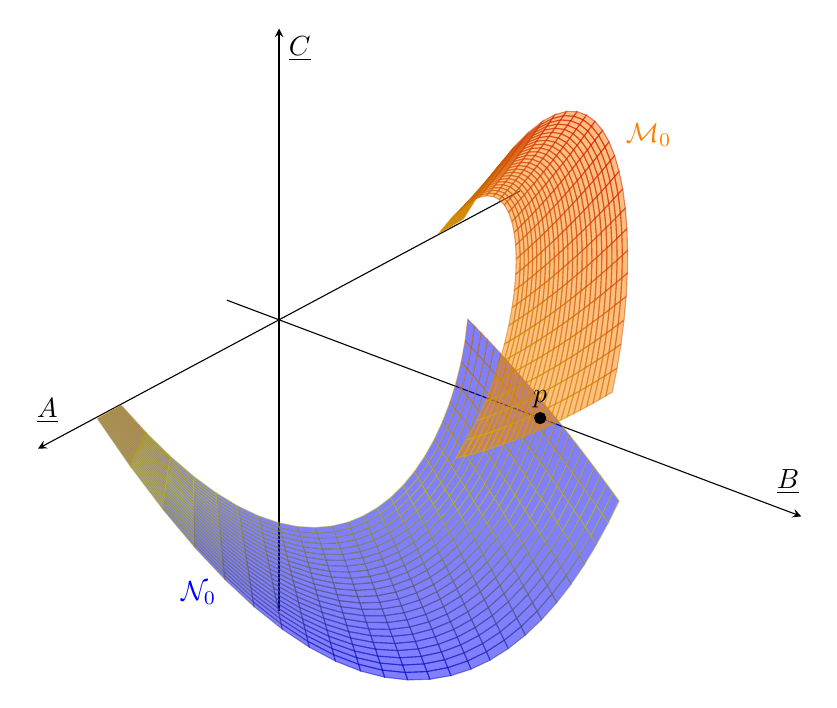
\begin{tikzpicture}
		\begin{axis}
			[
			axis lines = center,
			width=15cm,
			height=15cm,
			xmin = -1.0, xmax =1.0,
			ymin = -0.1, ymax= 1.0,
			zmin= -0.5, zmax=0.5,
			xtick style={draw = none},
			ytick style={draw = none},
			xticklabels={,,},
			yticklabels={,,},
			zticklabels={,,},
			ztick style={draw = none},
			xlabel=$\underline{A}$,
			ylabel=$\underline{B}$,
			zlabel=$\underline{C}$,
			view={130}{30},
			]
			\addplot3[surf,color= blue, opacity =0.5,
			domain=(0.7071 - 0.05 ):(0.7071 + 0.05), %omega
			domain y = 0.001:0.9, % t
			]
			({x*(1-y) - 0.1* y}, %
			{((-x^2 + 3*x^4 - (x*(1-y) - 0.1 * y)^2 + (x*(1-y) - 0.1 * y)^4 + 2*(x*(1-y) - 0.1 * 	y)*(x-2*x^3)))^(0.5)},
			{x - 2*x^3 - (x*(1-y) - 0.1 * y) + 2*(x*(1-y) - 0.1 * y)^3});
			\addplot3[surf,color= orange, opacity =0.5,
			domain=(-0.7071 - 0.05 ):(-0.7071 + 0.05), %omega
			domain y = 0.005:0.9, % t
			]
			({x*(1-y) + 0.1* y}, %
			{((-x^2 + 3*x^4 - (x*(1-y) + 0.1 * y)^2 + (x*(1-y) + 0.1 * y)^4 + 2*(x*(1-y) + 0.1 * y)*(x-2*x^3)))^(0.5)},
			{x - 2*x^3 - (x*(1-y) + 0.1 * y) + 2*(x*(1-y) + 0.1 * y)^3});
			\addplot3[mark=*,black,point meta=explicit symbolic,nodes near coords] 
			coordinates {(0,0.5,0)[$p$]};
			\addplot3[black,point meta=explicit symbolic,nodes near coords] 
			coordinates {(-0.45,0.5,0.35)[$\color{orange} {\mathcal M}_0$]};
			\addplot3[black,point meta=explicit symbolic,nodes near coords] 
			coordinates {(0.55,0.1,-0.35)[$\color{blue} {\mathcal N}_0$]};
		\end{axis}
	\end{tikzpicture}
	\caption{The above figure shows the stable and unstable manifolds for \(\epsilon = 0\). The manifolds \(\mathcal M_0\) and \(\mathcal N_0\) have a transverse intersection at \(p = (0,1/2,0)\).}
\end{figure}

Take \(\omega\) to be a point near \(A_{-\infty} = - 1/\sqrt 2\). For \(\epsilon = 0\), the orbit that approaches \((\omega, 0, 0)\) in backwards time lies on the intersection of 
\begin{equation*}
	\begin{aligned}
		I_1(\underline A, \underline B, \underline C) &= I_1(\omega, 0, 0) = \omega - 2\omega^3 \\
		I_2(\underline A, \underline B, \underline C) &= I_2(\omega, 0, 0) = - \frac 1 2 \omega^2 + \frac 3 2 \omega^4.
	\end{aligned}
\end{equation*}
Setting \(\underline A = 0\), we can find that \(\mathcal M_0\) hits the \(\underline B \underline C\)- plane at 
\begin{equation*}
	m(\omega) = (0, |\omega| \sqrt{3\omega^2 -1 }, \omega - 2\omega^3)
\end{equation*}
for \(\omega\) close to \(A_{-\infty}\). In particular, we see \(m(A_{-\infty}) = p\). Identical reasoning gives that \(\mathcal N_0\) intersects the plane at 
\begin{equation*}\label{intersection-with-plane}
	n(\alpha) = (0, |\alpha| \sqrt{3\alpha^2 -1 }, \alpha - 2\alpha^3)
\end{equation*}
where \(\alpha\) is near \(A_\infty = 1 / \sqrt 2\) and \(n (A_{\infty} ) = p\).

A tangent vector to the heteroclinic orbit is given by \(\gamma_{+}'(0) = (1/2, 0, -1/2)\), and this vector lies in both \(T_p\mathcal M_0\) and \(T_p \mathcal N_0\). Since \(m(\omega) \in \mathcal M_0\) for \(\omega\) near \(A_{-\infty}\), we have that 
\begin{equation*}
	m'(A_{-\infty}) = \left( 0, 1, \frac  1 {\sqrt 2} \right) \in T_p \mathcal M_0.
\end{equation*}
Similarly,
\begin{equation*}
	n'(A_{\infty}) = \left( 0, 1, \frac  {-1} {\sqrt 2} \right) \in T_p \mathcal N_0.
\end{equation*}
Therefore
\begin{equation*}
	T_p \mathcal M_0 + T_p \mathcal N_0 = \mathrm{span} \left\{ \left(\frac 1 2 , 0, \frac{-1} 2\right),  \left( 0, 1, \frac  1 {\sqrt 2} \right) ,  \left( 0, 1, \frac  {-1} {\sqrt 2} \right) \right\} = T_p\R^3
\end{equation*}
and the intersection is transverse. This implies that there is a heteroclinic orbit on the intersection of \(\mathcal M_\epsilon\) and \(\mathcal N_\epsilon\) for \(\epsilon > 0\) (see \cite[Chp.~6]{arnold1988geometrical} for details). 


\subsection{Estimates on the heteroclinic orbit}

From the previous section, we have the existence of heteroclinic orbits that are perturbation of \(\gamma_\pm\) at \(\epsilon = 0\). From the \(C^1\) regularity of the manifolds with respect to the coordinates, we expect that the orbits remain \(\mcO(\epsilon)\) close to the unperturbed orbits in some sense. There are some subtleties to be addressed. The manifolds remain \(\mcO(\epsilon)\) close in Hausdorff distance, but this does not imply the orbits on the manifolds remain \(\mcO(\epsilon)\) close for all time. The dynamics on the manifolds might change causing orbits on the perturbed manifold to diverge asymptotically despite remaining close initially.

First, let us introduce notation for the perturbed heteroclinic orbits. We shall denote by \(\gamma_{\pm, \epsilon} = (A_{\pm, \epsilon} , B_{\pm, \epsilon}, C_{\pm,\epsilon})\) the perturbations of \(\gamma_{\pm}\) for \(\epsilon > 0\), where we set \(\gamma_{\pm,\epsilon}(0)\) to be the point where the orbits cross the \(\underline{B}\underline{C}\)-plane. From the continuity of the manifolds with respect to \(\epsilon\), we have that \(|\gamma_{\pm, \epsilon}(0) - \gamma_\pm(0)| = \mcO(\epsilon)\) for small \(\epsilon\). We can extend this estimate onto arbitrarily large finite time scales by applying an argument using the Gr\"onwall inequality. That is, for every \(T> 0\) we have for sufficiently small \(\epsilon\) that \(|\gamma_{\pm, \epsilon}(s) - \gamma_\pm(s)| = C\epsilon\) for all \(s\in[-T,T]\), where \(C>0\) is independent of \(s\). 

This argument is insufficient for extending the estimate to all time. To get that the orbits remain close as \(s\to\pm\infty\), we can rely on part 7 of \cref{foliation-of-unstable-manifold}. Checking the values of the generalized Lyapunov-type numbers, we can see that at \(p = (A_{-\infty}, 0, 0, 0)\), we have that
\begin{equation*}
	\sigma^{cu}(p_0) = \exp(-\sqrt{6 A_{-\infty}^2 -1}), \quad \sigma^{su}(p_0) = \exp(-2\sqrt{6 A_{-\infty}^2 -1}).
\end{equation*}
Then if we make the manifold small enough, this condition for the hypotheses of \cref{foliation-of-unstable-manifold} hold. We check that this condition is not broken by perturbation of the vector field with the bump function in \cref{condition-verification}. Taking \((\epsilon, \omega)\) sufficiently close to \((0, A_{-\infty})\) as base points, the theorem states that the unstable manifold is \(C^1\) with respect to \((\epsilon, \omega)\). Note that the overflowing invariant manifold (away from the bump function) consists only of fixed points, so orbits on the unstable manifold approach a unique fixed point given by \((\epsilon, \omega)\). Take \(T> 0\) large enough so that all the points on \(\mathcal M_\epsilon\) (for \(\epsilon \leq \epsilon_0\)) which intersect the \(\underline B \underline C\)-plane are in the local unstable manifold when flowed backward in time by \(-T\) units. Then locally, there is a one-to-one correspondence between these points flowed backward in time and the points in \(\overline M\); furthermore, this correspondence is \(C^1\) due to \cref{foliation-of-unstable-manifold}. This implies that if the points flowed backward are \(\mcO(\epsilon)\) close then their backward limits are \(\mcO(\epsilon)\) close as well. In particular, the backward limits of \(\gamma_{+,\epsilon}\) and \(\gamma_+\) are \(\mcO(\epsilon)\) close. The argument for the stable manifold is analogous. This shows that the heteroclinic orbits remain \(\mcO(\epsilon)\) close for all time. In the case where \(V(x) = \frac 12 x^2 - \frac 1 {24} x^4 + \mcO(\epsilon^6)\), this can be upgraded to \(\mcO(\epsilon^2)\); the proof is similar but we use the regularity of the manifolds with respect to \(\eta = \epsilon^2\) instead. Therefore, we have the following.
\begin{prop}
	There exists \(\epsilon_0 > 0\) such that for every \(\epsilon\in(0,\epsilon_0]\) there exist two heteroclinic orbits \(\gamma_{\pm, \epsilon}\) of \cref{epsilon-flow} such that 
	\begin{equation*}
		|\gamma_{\pm,\epsilon}(s) - \gamma_\pm(s) | \leq C \epsilon \quad \text{ for all } s\in \R
	\end{equation*}
	where \(\gamma_{\pm}\) are defined in \cref{heteroclinic-orbit-at-zero}. If \(V\) satisfies (H2), then we instead have the estimate
	\begin{equation*}
		|\gamma_{\pm,\epsilon}(s) - \gamma_\pm(s) | \leq C \epsilon^2 \quad \text{ for all } s\in \R.
	\end{equation*}
\end{prop}

By starting to unravel the change of coordinates, we can show the existence of solutions to the advance-delay equation of the form
\begin{equation*}
	x_{\pm,\epsilon}(t) = q_{\pm, \epsilon}(t) + (\Phi_\mu(\epsilon A_{\pm, \epsilon}(\epsilon t),\epsilon^2 B_{\pm, \epsilon}(\epsilon t) ,\epsilon^3 C_{\pm, \epsilon}(\epsilon t))_x
\end{equation*}
where \(q_{\pm, \epsilon}(t)\) satisfies the differential equation
\begin{equation*}
	\frac{dq_{\pm, \epsilon}}{dt} =  \epsilon A_{\pm, \epsilon}(\epsilon t).
\end{equation*}
The differential equation for \(q\) comes from \cref{ode-for-q} and the fact that \(\zeta_1^*(\Phi_\mu) = 0\). Using the fact that for solutions of \cref{first-order-abstract-ode} satisfy \(\partial_t (U)_x = U_\xi\), we also have that
\begin{equation*}
	\dot x_{\pm, \epsilon}(t) =  \epsilon A_{\pm, \epsilon}(\epsilon t) + (\Phi_\mu(\epsilon A_{\pm, \epsilon}(\epsilon t),\epsilon^2 B_{\pm, \epsilon}(\epsilon t) ,\epsilon^3 C_{\pm, \epsilon}(\epsilon t))_\xi.
\end{equation*}
The coordinates \(A_{\pm, \epsilon}\), \(B_{\pm, \epsilon}\), and  \(C_{\pm, \epsilon}\) are at least \(C^5\) and \(\Phi_\mu\) is at least \(C^4\) in its spatial variables.

The main result will be stated by writing \cref{fput-lattice-odes} in terms of the strain variables, \(u_n = x_{n+1} - x_n\). That is, we look at the traveling wave solution given by 
\begin{equation*}
	x_{\pm, \epsilon}(n+1-c\tilde t) - x_{\pm, \epsilon}(n-c\tilde t).
\end{equation*}
Using a Taylor series expansion centered at \(t + \frac 12 \) for \( x_{\pm, \epsilon}(t+ 1)\) and \( x_{\pm, \epsilon}(t)\), we get 
\begin{align}
	& x_{\pm, \epsilon}(t+ 1/2) + \frac 12 \dot x_{\pm, \epsilon}(t+1/2) + \frac 1 8\ddot x_{\pm, \epsilon}(t+1/2) + \frac 1 2\int_{0}^{1/2} \dddot x_{\pm, \epsilon}(t+1/2+s)(s-1/2)^2 \, ds \\
	& x_{\pm, \epsilon}(t+ 1/2) - \frac 12 \dot x_{\pm, \epsilon}(t+1/2) + \frac 1 8 \ddot x_{\pm, \epsilon}(t+1/2) - \frac 1 2\int_0^{1/2} \dddot x_{\pm, \epsilon}(t+s)s^2 \, ds 
\end{align}
respectively for each term. Thus 
\begin{equation*}
\begin{aligned}
	&x_{\pm, \epsilon}(t+1) - x_{\pm, \epsilon}(t) \\
	&\quad= \dot x_{\pm, \epsilon}(t+ 1/2) + \frac 12 \int_{0}^{1/2} [\dddot x_{\pm, \epsilon}(t+1/2+s)(s-1/2)^2 - \dddot x_{\pm, \epsilon}(t+s)s^2] ds \\
	&\quad= \pm \epsilon \varphi_1(\epsilon (t+1/2)) + \epsilon^2 \mathcal R_{\epsilon, \pm}(\epsilon (t+1/2))
\end{aligned}
\end{equation*}
where \(R_{\epsilon, \pm} \in C^3_b\). Thus (after shifting the solution) we have that there are traveling wave like solutions of the FPUT of the form
\begin{equation*}
	u_n(t) = \pm \epsilon \varphi_1(\epsilon(n-ct)) + \epsilon^2 \mathcal R_{\epsilon, \pm}(\epsilon (n-ct))
\end{equation*}
Additionally, if (H2) holds we improve the error estimate so that there are solutions of the form 
\begin{equation*}
	u_n(t) = \pm \epsilon \varphi_1(\epsilon(n-ct)) + \epsilon^3 \mathcal R_{\epsilon, \pm}(\epsilon (n-ct)).
\end{equation*}

To match similar estimates made in \cite{friesecke1999solitary}, one would expect the remainder terms to also be in a Sobolev space like \(H^1\). This is in general not true. The traveling wave solution found above may approach a different limit asymptotically than \(\epsilon \varphi_1 \), in which case the remainder does not approach zero asymptotically in space. A necessary condition to get \(\mathcal R_{\epsilon,\pm}\in H^1\) would be for \(u_n\) to approach the same limits of \(\pm \epsilon \varphi_1(\epsilon (n-ct))\) as \(|n| \to \infty\).

A useful tool for showing this is the following invariant for \cref{advance-delay-equation}:
\begin{equation}\label{advance-delay-invariant}
	\dot x(t) - \mu \int_t^{t+1} V'(x(s) - x(s-1)) \, ds.
\end{equation}
It is easy to check that the above is constant for solutions of the advance-delay differential equation. If \(\dot x(t) \to r_\infty\) as \(t\to \infty\), then \cref{advance-delay-invariant} is equal to 
\begin{equation*}
	r_\infty - \mu V'(r_\infty)
\end{equation*}
If we also have that \(\dot x(t) \to r_{-\infty}\) as \(t\to-\infty\), then we have \cref{advance-delay-invariant} is also equal to 
\begin{equation*}
	r_{-\infty} - \mu V'(r_{-\infty}) 
\end{equation*}
and so the limits \(r_{\pm \infty}\) satisfy the equation
\begin{equation*}
	r_\infty - \mu V'(r_\infty) = r_{-\infty} - \mu V'(r_{-\infty}) .
\end{equation*}
For arbitrary \(V\), we cannot show that the limits agree with the limits of \(\pm\epsilon \phi \). However, if we assume (H3) holds, i.e.\ that \(V(x) = \frac 1 2 x^2 - \frac 1 {24} x^4\), then we do have the limits agree. This follows in part from the oddness of \(V'\) and the reversibility of the system. Recall that the vector field on the center manifold is reversible (given by the reversibility operator \(S_0\)) and odd. Therefore, we have that
\begin{equation*}
	\begin{bmatrix}
		- A_{\pm, \epsilon} (-s) \\
		B_{\pm, \epsilon} (-s) \\
		-C_{\pm, \epsilon} (-s)
	\end{bmatrix}
\end{equation*}
is also a solution on the center manifold. One can note that the above solutions lie on the intersection of the stable and unstable manifolds and are in an \(\epsilon\)-neighborhood of the unperturbed heteroclinic orbits \(\gamma_{\pm}(s)\). This contradicts the uniqueness of the transverse intersection of the manifolds in a neighborhood of the original intersection, and thus the above solutions must in fact be \(\gamma_{\pm,\epsilon}(s)\). Hence, comparing the limits at infinity we have that \(\lim_{s\to\infty} A_{\pm,\epsilon} (s) = -\lim_{s\to-\infty} A_{\pm, \epsilon}(s)\) and so \(r_\infty = - r_{-\infty}\). Therefore, we must have that 
\begin{equation*}
	r_\infty - \mu V'(r_\infty) = 0.
\end{equation*}
Given that \(V'(x) = x - \frac 1 6 x^3\), we have that the only solutions to the above equation are \(r_{\infty} = 0, \pm \epsilon / \sqrt 2\). This implies that the limits of the traveling wave solutions agree with \(\pm \epsilon \phi\). Specifically, we must have \(A_{\pm, \epsilon}(s) \to \pm 1 / \sqrt 2\) as \(s\to \infty\) and \(A_{\pm, \epsilon}(s) \to \mp 1 / \sqrt 2\) as \(s\to -\infty\).

Now to get the Sobolev estimate, we use the following lemma.
\begin{restatable}{lem}{heteroclinicorbitsobolev}\label{heteroclinic-orbit-sobolev}
	Suppose that (H3) holds. Then there exist \(C> 0\) and \(\alpha > 0\) such that
	\begin{equation*}
		| \gamma_{\pm, \epsilon}(s) - \gamma_{\pm}(s) | \leq C e^{-\alpha| s|} \epsilon.
	\end{equation*}
	Furthermore, the difference of the heteroclinic orbits are in \(H^5(\R; \R^3)\) and 
	\begin{equation*}
		\| \gamma_{\pm, \epsilon}(s) - \gamma_{\pm}(s) \|_{H^5(\R;\R^3)}  \leq C \epsilon.
	\end{equation*}
\end{restatable}
The proof of \cref{heteroclinic-orbit-sobolev} is given in \cref{lemma-appendix}. Thus we have
\begin{equation*}
	\|A_{\pm, \epsilon} \mp \varphi_{1}\|_{H^5(\R;\R)} \leq C \epsilon.
\end{equation*}
One can also show from the exponential decay of \(\gamma_{\pm, \epsilon}\) and the smoothness of \(\Phi_\mu\) that
\begin{equation*}
	(\Phi_\mu(\epsilon A_{\pm, \epsilon}(s),\epsilon^2 B_{\pm, \epsilon}(s) ,\epsilon^3 C_{\pm, \epsilon}(s))_\xi \in H^4(\R;\R).
\end{equation*}
By noticing that the Taylor expansion of \(\Phi_\mu(\epsilon A_{\pm, \epsilon}, \epsilon^2 B_{\pm, \epsilon}, \epsilon^3 C_{\pm, \epsilon})\) has no terms of order \(\epsilon^2\) or lower, the function is at least of order \(\epsilon^3\). Therefore, we have that there is an \(R_{\pm,\epsilon} \in H^4(\R;\R)\) such that
\begin{equation*}
	\dot x_{\pm, \epsilon }(t) = \pm \epsilon\varphi_1(\epsilon t) + \epsilon^2 R_{\pm,\epsilon}(\epsilon t).
\end{equation*}
Then converting to strain coordinates as before we have
\begin{equation*}
	u_n(t) = \pm\epsilon\varphi_1(\epsilon(n-ct)) + \epsilon^2 \mathcal R_{\pm, \epsilon}(\epsilon(n-ct))
\end{equation*}
where \(\mathcal R_{\pm, \epsilon} \in H^3(\R;\R)\).

We state our results as follows.
\begin{theorem}\label{thm:estimates-on-profile}
	There exists \(\epsilon_0> 0\) and \(C> 0\) such that for every \(\epsilon > (0,\epsilon_0]\) there is a traveling wave solution given by \(u_n(t) = u_c(n-ct)\) with positive wave speed \(c^2 = 1 - \epsilon^2/12\). Furthermore, we have the additional estimates on the wave profile of \(u_c\).
	\begin{enumerate}[label = (\roman*)]
		\item If (H1) holds, then
		\begin{equation*}
			\left\| \frac 1 \epsilon u_c\left(\frac \cdot \epsilon \right) - \varphi_1 \right\|_{C^3} \leq C \epsilon
		\end{equation*}
		\item If (H2) holds, then
		\begin{equation*}
			\left\| \frac 1 \epsilon u_c\left(\frac \cdot \epsilon \right) - \varphi_1 \right\|_{C^3} \leq C \epsilon^2
		\end{equation*}
		\item If (H3) holds, then
		\begin{equation*}
			\left\| \frac 1 \epsilon u_c\left(\frac \cdot \epsilon \right) - \varphi_1 \right\|_{H^3} \leq C \epsilon
		\end{equation*}
	\end{enumerate}
\end{theorem}
The same estimates hold for \(-\varphi_1\) as the profile wave or for left-moving waves or for both.